% fig1_pipeline.tex -- scCausal framework overview (mechanism schematic, no result claims)
%
% DESIGN CONTRACT (Nature Research figure guide, "Preparing figures")
%   * sans-serif Helvetica throughout
%   * body text 6-7 pt AT FINAL PRINT SIZE  -> canvas drawn at 1:1
%     canvas 16.30 x 7.10 cm; \textwidth of cas-sc = 16.46 cm -> scale ~1.00
%   * no coloured text: colour lives only in fills, rules and arrows
%   * flat design: hairline borders, no drop shadow, no gradient
%   * colourblind-safe: single blue accent + one green accent
%   * stage badges 6 pt bold white on filled disc
%
% GEOMETRY (cm), canvas 16.30 wide x 7.10 tall
%   boxes w=3.25 h=3.80, gaps 0.90, side margins 0.30
%     B1 0.30-3.55 (c=1.925)   B2 4.45-7.70 (c=6.075)
%     B3 8.60-11.85 (c=10.225) B4 12.75-16.00 (c=14.375)
%   gaps centred at 4.00 / 8.15 / 12.30 ; boxes span y 1.20-5.00 (c=3.10)
\documentclass[tikz,border=2pt]{standalone}
\usepackage[T1]{fontenc}
\usepackage{fix-cm}% CM at arbitrary sizes -> no font-substitution warnings for 6.5 pt math
\usepackage{helvet}
\usepackage{amsmath,amssymb}
\usepackage{xcolor}
\usepackage{tikz}
\usetikzlibrary{arrows.meta, calc, backgrounds}
\renewcommand{\familydefault}{\sfdefault}

\definecolor{ink}{HTML}{1F2933}      % all text
\definecolor{muted}{HTML}{5C6B76}    % secondary text
\definecolor{rule}{HTML}{D3DCE3}     % hairline neutrals
\definecolor{blue}{HTML}{1B6CA8}
\definecolor{bluefill}{HTML}{EFF5FA}
\definecolor{blueline}{HTML}{AFCBE0}
\definecolor{green}{HTML}{0E7C66}
\definecolor{greenfill}{HTML}{ECF6F2}
\definecolor{greenline}{HTML}{A5D0C4}
\definecolor{arrowc}{HTML}{46545F}

\begin{document}
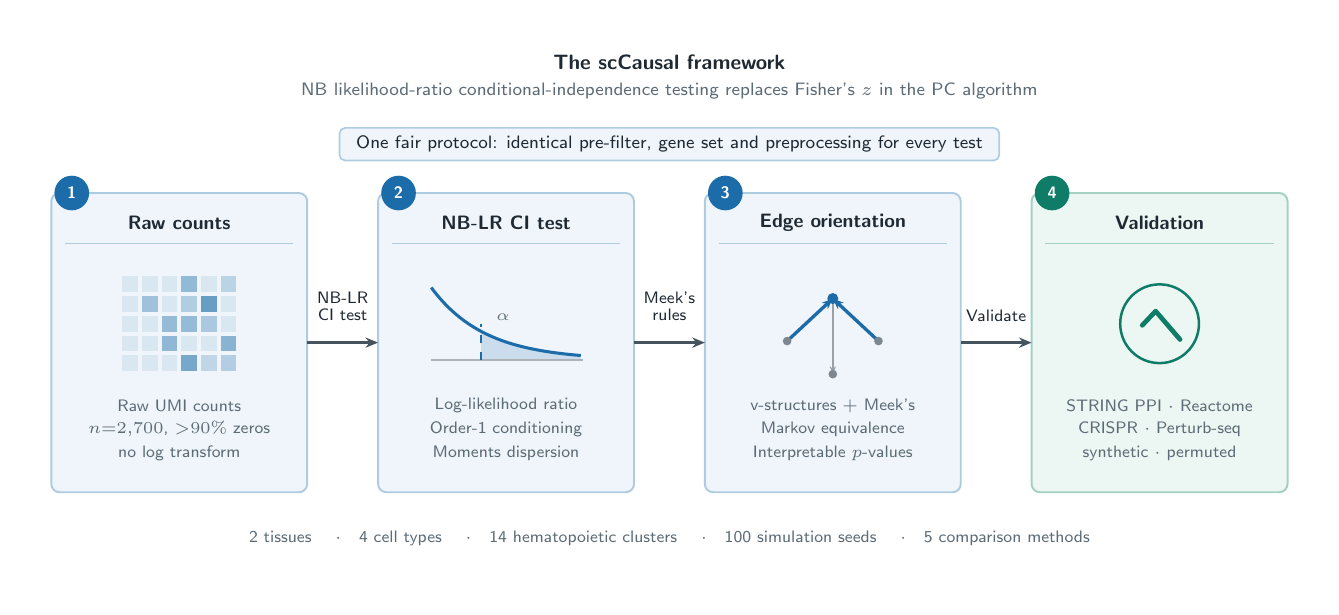
\begin{tikzpicture}[
    ebox/.style={rectangle, rounded corners=3pt, line width=0.7pt,
                 inner sep=0pt, minimum width=3.25cm, minimum height=3.80cm},
    badge/.style={circle, inner sep=0pt, minimum size=4.4mm,
                  font=\fontsize{6}{7}\selectfont\bfseries, text=white},
    flow/.style={-{Stealth[length=1.6mm,width=1.3mm]}, line width=1.0pt, draw=arrowc},
    glab/.style={font=\fontsize{6}{7}\selectfont, text=ink, align=center},
    dline/.style={font=\fontsize{6}{7.2}\selectfont, text=muted, align=center},
]

% force the exact canvas so the printed scale is known
\path[use as bounding box] (0,0) rectangle (16.30,7.10);

% ======================= HEADER =======================
\node[font=\fontsize{7.5}{9}\selectfont\bfseries, text=ink, align=center]
    at (8.15, 6.66) {The scCausal framework};
\node[font=\fontsize{6.5}{8}\selectfont, text=muted, align=center]
    at (8.15, 6.30)
    {NB likelihood-ratio conditional-independence testing replaces Fisher's $z$ in the PC algorithm};

% fair-protocol strip: the paper's methodological contribution, not a result
\node[rounded corners=2pt, draw=blueline, line width=0.6pt, fill=bluefill,
      inner xsep=6pt, inner ysep=3pt, font=\fontsize{6.5}{8}\selectfont,
      text=ink, align=center] at (8.15, 5.62)
    {One fair protocol: identical pre-filter, gene set and preprocessing for every test};

% ======================= STAGE 1 : RAW COUNTS =======================
\node[ebox, draw=blueline, fill=bluefill] (b1) at (1.925, 3.10) {};
\node[badge, fill=blue] at (0.56, 5.00) {1};
\node[font=\fontsize{7}{8.5}\selectfont\bfseries, text=ink] at (1.925, 4.62) {Raw counts};
\draw[blueline, line width=0.6pt] (0.475, 4.36) -- (3.375, 4.36);
% heatmap icon (seeded -> reproducible)
\begin{scope}[shift={(1.925, 3.32)}]
  \pgfmathsetseed{42}
  \foreach \r in {1,...,5}{
    \foreach \c in {1,...,6}{
      \pgfmathsetmacro{\q}{random(0,100)}
      \pgfmathsetmacro{\op}{max(0.10, 0.32+(\q-58)/42*0.6)}
      \pgfmathsetmacro{\xoff}{-0.725+(\c-1)*0.25}
      \pgfmathsetmacro{\yoff}{0.62-(\r-1)*0.25}
      \fill[blue, fill opacity=\op] (\xoff,\yoff) rectangle ++(0.20,-0.20);
    }}
\end{scope}
\node[dline] at (1.925, 2.30) {Raw UMI counts};
\node[dline] at (1.925, 2.00) {$n{=}2{,}700$, ${>}90\%$ zeros};
\node[dline] at (1.925, 1.70) {no log transform};

% ======================= STAGE 2 : CI TEST =======================
\node[ebox, draw=blueline, fill=bluefill] (b2) at (6.075, 3.10) {};
\node[badge, fill=blue] at (4.71, 5.00) {2};
\node[font=\fontsize{7}{8.5}\selectfont\bfseries, text=ink] at (6.075, 4.62) {NB-LR CI test};
\draw[blueline, line width=0.6pt] (4.625, 4.36) -- (7.525, 4.36);
% chi-square null with shaded upper tail (schematic, no data)
\begin{scope}[shift={(6.075, 3.32)}]
  \fill[blue, fill opacity=0.17]
      plot[domain=1.5:4.5, samples=45] (\x*0.4222-0.95, {exp(-\x*0.62)*0.92-0.44})
      -- (0.95,-0.44) -- (-0.317,-0.44) -- cycle;
  \draw[arrowc!45, line width=0.6pt] (-0.95,-0.44) -- (0.98,-0.44);
  \draw[blue, line width=1.1pt, domain=0:4.5, samples=50]
      plot (\x*0.4222-0.95, {exp(-\x*0.62)*0.92-0.44});
  \draw[blue, dashed, line width=0.7pt] (-0.317,-0.44) -- (-0.317,0.02);
  \node[anchor=west, font=\fontsize{5.5}{6.5}\selectfont, text=muted]
      at (-0.25, 0.10) {$\alpha$};
\end{scope}
\node[dline] at (6.075, 2.30) {Log-likelihood ratio};
\node[dline] at (6.075, 2.00) {Order-1 conditioning};
\node[dline] at (6.075, 1.70) {Moments dispersion};

% ======================= STAGE 3 : ORIENTATION =======================
\node[ebox, draw=blueline, fill=bluefill] (b3) at (10.225, 3.10) {};
\node[badge, fill=blue] at (8.86, 5.00) {3};
\node[font=\fontsize{7}{8.5}\selectfont\bfseries, text=ink] at (10.225, 4.62) {Edge orientation};
\draw[blueline, line width=0.6pt] (8.775, 4.36) -- (11.675, 4.36);
% DAG icon; the v-structure converging on the bottom node is highlighted
% collider (v-structure) A -> C <- B, plus one outgoing oriented edge C -> D
\begin{scope}[shift={(10.225, 3.36)}]
  \coordinate (A) at (-0.58,-0.24);
  \coordinate (B) at ( 0.58,-0.24);
  \coordinate (C) at ( 0.00, 0.30);
  \coordinate (D) at ( 0.00,-0.66);
  \draw[arrowc!55, line width=0.6pt, -{Stealth[length=1.0mm,width=0.8mm]}]
      (C) -- (D);
  \draw[blue, line width=1.2pt, -{Stealth[length=1.4mm,width=1.1mm]}] (A) -- (C);
  \draw[blue, line width=1.2pt, -{Stealth[length=1.4mm,width=1.1mm]}] (B) -- (C);
  \foreach \n in {A,B,D}{\fill[arrowc!70] (\n) circle (0.055);}
  \fill[blue] (C) circle (0.070);
\end{scope}
\node[dline] at (10.225, 2.30) {v-structures $+$ Meek's};
\node[dline] at (10.225, 2.00) {Markov equivalence};
\node[dline] at (10.225, 1.70) {Interpretable $p$-values};

% ======================= STAGE 4 : VALIDATION =======================
\node[ebox, draw=greenline, fill=greenfill] (b4) at (14.375, 3.10) {};
\node[badge, fill=green] at (13.01, 5.00) {4};
\node[font=\fontsize{7}{8.5}\selectfont\bfseries, text=ink] at (14.375, 4.62) {Validation};
\draw[greenline, line width=0.6pt] (12.925, 4.36) -- (15.825, 4.36);
% line-art check in a ring
\begin{scope}[shift={(14.375, 3.34)}]
  \draw[green, line width=0.9pt] (0,0) circle (0.50);
  \draw[green, line width=1.7pt, line cap=round, line join=round]
      (-0.22,-0.02) -- (-0.05,0.16) -- (0.26,-0.20);
\end{scope}
\node[dline] at (14.375, 2.30) {STRING PPI $\cdot$ Reactome};
\node[dline] at (14.375, 2.00) {CRISPR $\cdot$ Perturb-seq};
\node[dline] at (14.375, 1.70) {synthetic $\cdot$ permuted};

% ======================= FLOW ARROWS =======================
\draw[flow] (3.55, 3.10) -- (4.45, 3.10);
\node[glab] at (4.00, 3.56) {NB-LR\\[-1pt]CI test};
\draw[flow] (7.70, 3.10) -- (8.60, 3.10);
\node[glab] at (8.15, 3.56) {Meek's\\[-1pt]rules};
\draw[flow] (11.85, 3.10) -- (12.75, 3.10);
\node[glab] at (12.30, 3.44) {Validate};

% ======================= FOOTER =======================
\node[font=\fontsize{6}{7}\selectfont, text=muted, align=center] at (8.15, 0.62)
    {2 tissues \quad$\cdot$\quad 4 cell types \quad$\cdot$\quad 14 hematopoietic clusters \quad$\cdot$\quad 100 simulation seeds \quad$\cdot$\quad 5 comparison methods};

\end{tikzpicture}
\end{document}
